\subsection{Toy model}

Assume that we have two agents: Alice, a service provider, and Bob, a service requester. 
For a generic service, Bob will pay Alice $p$ each period.
The generic service will typically imply a requirement that the value of the funds involved in the service it itself `insured'.
For instance, Bob may enlist Alice to perform an atomic swap for funds of total value $V$, offering a payment $p$ for this service, where $p<V$.
Alice has options, as follows.

\begin{enumerate}
    \item[A:] post collateral $D$ upfront, such that $D=V$
    \item[B:] accrue collateral by saving payments $p$ each time period $t$
\end{enumerate}

The constraint is that Alice is not able to offer a service for a value larger than the sum of the collateral that she has in escrow. 
In the first case, Alice is able to offer a service of a value equal to the amount of posted collateral, $D$.
In the second case, the insured value is equal to the cumulative sum of the payments received.

While (A) offers users insurance of a larger transaction volume immediately, it involves a high capital burden on Alice, who must post collateral equal to the total value $V$. 
In contrast, (B) enables Alice to use the received payments $p$ as collateral, with the \textit{promise} that the sum of payments to Alice are sufficient to ensure full collateralization, previous payments will be made to Alice directly.
This eases the upfront collateral burden on Alice.

\begin{figure}
    \centering
    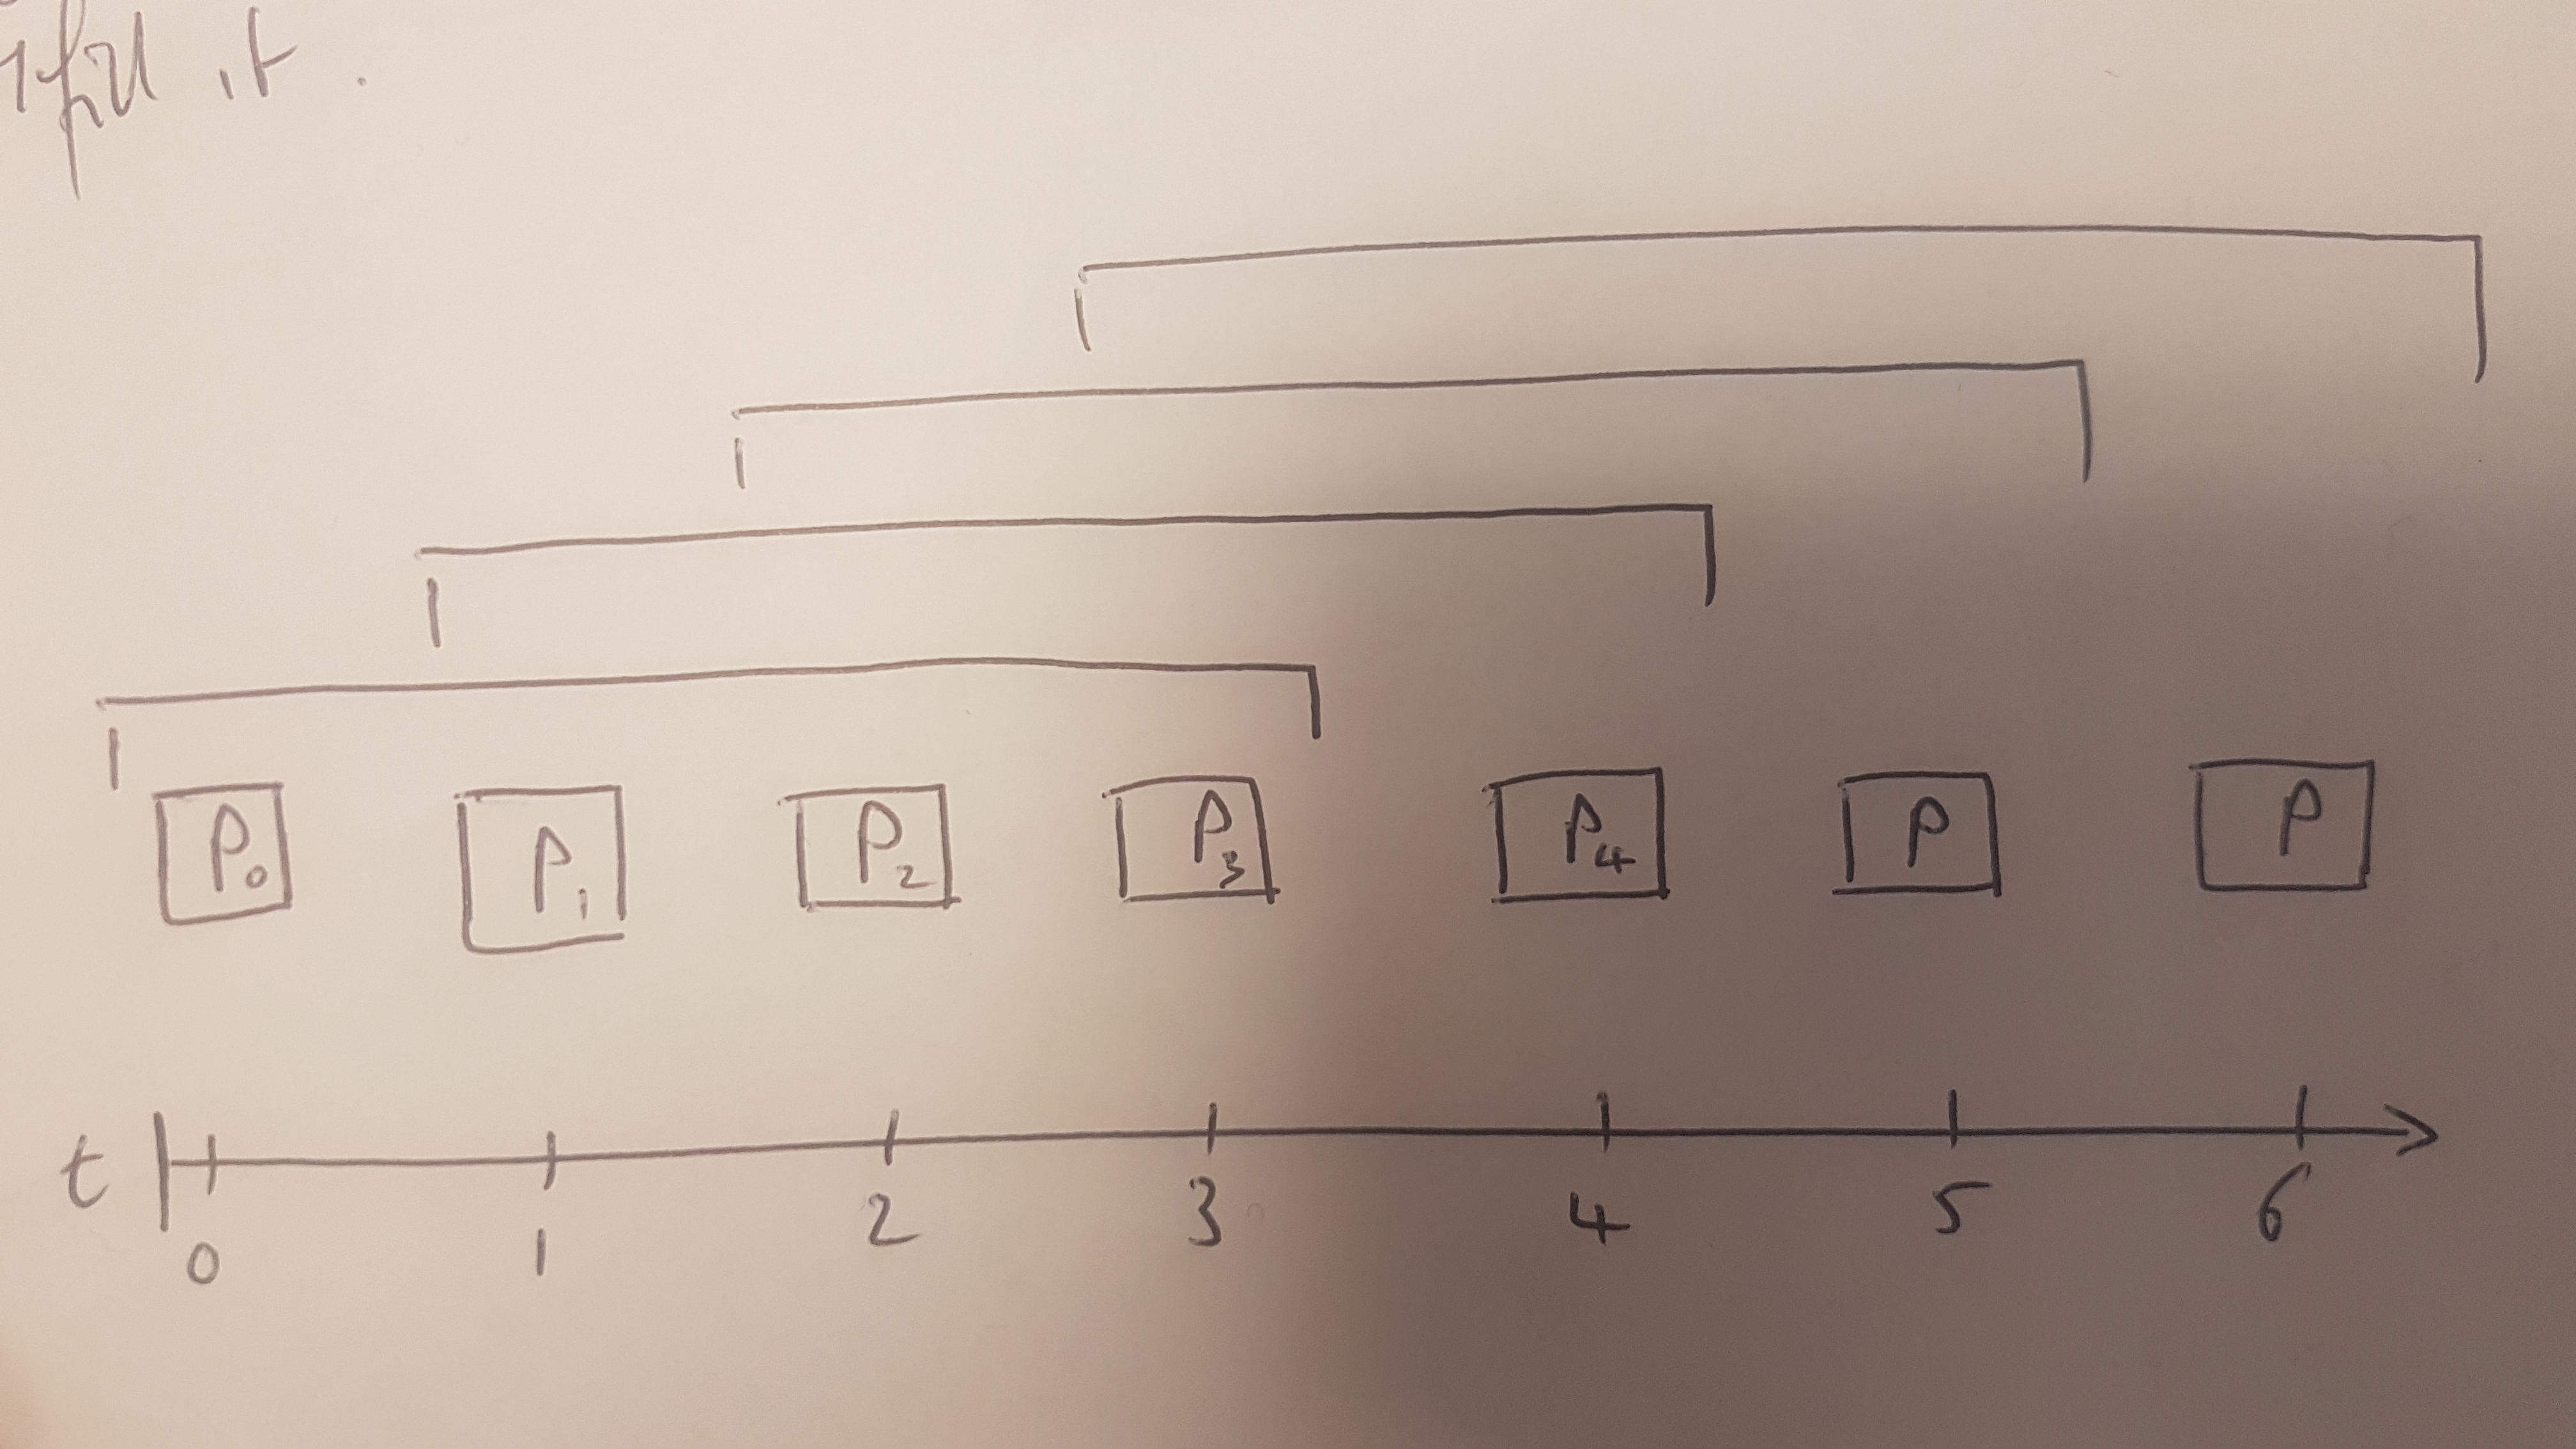
\includegraphics[width=\textwidth]{promise/figures/slidingwindows.jpg}
    \caption{Figure showing the mechanics of the sliding window.}
    \label{fig:slidingwindows}
\end{figure}

Alice decides to eventually offer collateral equivalent to $S=4$ periods of stored payments (from $t=0$ to $t=3$).
Therefore, until $t=4$, she does not receive any payment. 
At $t=4$, she receives payment $p$, which discounted is $(\frac{\delta}{1+r})^4$.
Similarly, at $t=5$, she receives another payment $p$, worth $(\frac{\delta}{1+r})^5$ to Alice today.
At the same time, Alice accrues opportunity costs of the locked funds ($p$) per period.
Alice incurs an opportunity cost of $\mathrm{E}[r]p$ in the first period, $\mathrm{E}[r](2p)(\frac{\delta}{1+r})$ in the second period, etc. 

If Alice offers such a service indefinitely, the total value of this, $T_v$, for a single iteration, is as follows. 

\begin{equation}
\label{eq:payoffs_longform}
T_v=(\frac{\delta}{1+r})p-\mathrm{E}[r](p+2p(\frac{\delta}{1+r})+3p(\frac{\delta}{1+r})^2+4p(\frac{\delta}{1+r})^3)
\end{equation}

Iterating $k$ times, the total net present value of $T_v$ is:

\begin{equation}
\label{eq:payoffs_longform}
T_v=\sum_{k=0}^{\infty}(\frac{\delta}{1+r})^{S+k}p-\mathrm{E}[r]p\sum_{k=0}^{\infty}(\frac{\delta}{1+r})^k(\sum_{i=0}^{S-1}(i+1)(\frac{\delta}{1+r})^i)
\end{equation}

\lgu{From here, maybe we want to compare to the status quo, where the operator fronts all the collateral upfront.
We would find that since the system `ramps up', the opportunity costs would be lower in the beginning, but this isn't that interesting because at the same time the service level is worse (only insured up to the cumulative total). So really what we are presenting is a funding model for cryptoeconomic protocols, where the operator's collateral is made up of user payments until some threshold cumulative total is reached? We could argue that this is valuable because it allows operators to get started?}

\dom{I agree with you. So in essence the cost of the locked collateral is reduced until you reach $t=4$ in the model above. Overall, it helps you bootstrap your system and allows your intermediaries to accumulate the required collateral. What I'm wondering is, if you have the same motivation to not cheat with the lower collateral in the beginning. I guess here we need to argue in a different way from the Balance paper. In Balance we say that $p=0$ and than argue that the proofs still hold. Here we need to assume that $p>0$ and perfect competition does not exist. This needs to go into the security discussion.}


\section{Model as of 18 September}

\subsection{The setup}

Consider the following setup.

\begin{itemize}
    \item an operator, Alice, who can offer a collateralized service for off-chain payments. This service can offer a varying degree of instant finality. 
    \item $n$ users, including Bob, who wish to make and receive payments. 
    \item each user pays a fee $p$ per inbound transaction (assumed to be the same size each period for simplicity.
\end{itemize}

Alice has a choice between two actions: acting honestly, or cheating. 
With \sys, the payoffs to Alice of each of these actions are as follows.
Assume that any cheating happens at period $t=T$.

\dom{Why is the deposit added to the payoff when being honest? Before the protocol started, the deposit was already in the account of the operator. So his net profit is only the payment.}
\begin{equation}
\label{eq:promise_honest}
\Pi_H = D(\frac{\delta}{1+r})^T+p\sum^{T}_{t=0}(\frac{\delta}{1+r})^t
\end{equation}

\dom{Why do you subtract the payment from the payoff for cheating? Before the protocol started, the operator did not have the payment in his account. He will not receive the payment, but that does not mean that he has to pay an amount equal to the payment into the system.}

\begin{equation}
\label{eq:promise_cheat}
\Pi_C = V-D(\frac{\delta}{1+r})^T-p\sum^{T}_{t=0}(\frac{\delta}{1+r})^t
\end{equation}


\dom{
Let's take an example where Alice (operator) starts with a balance of 10 ETH and Bob starts with a balance of 10 ETH and has multiple goods with value 15 ETH each. 
For simplicity, I will not consider any discount factors or opportunity costs.
Bob is willing to pay Alice 1 ETH per transaction, i.e. one transfer of the good.
In the first of those transaction Alice posts 10 ETH as collateral, she now has a balance of 0 ETH (-D).
Bob then pre-pays 10 ETH to pay for the transactions. Bob has a balance of 0 ETH (-q).
The escrow contract has 20 ETH now.
Alice has two choices.
\begin{itemize}
    \item Honest: Alice is honest and the good is transferred successfully. Alice and Bob still have 0 ETH in their accounts. If we would finish the transactions at this point, Alice would get her deposit back and the payment for one transaction (even after some time) and Bob would get the remainder from his pre-payment out. Alice would have 11 ETH and Bob 9 ETH. \textbf{Alice went from 10 ETH to 11 ETH. The equation for honest behaviour is therefore $u = p$ (or $\Pi_H=p$ in the notation above).}. Again without considering the discount factor. Alice does not get any surplus deposit.
    \item Cheating: Alice decides to steal the good from Bob. Alice and Bob still have 0 ETH in their accounts. Let's say Alice is able to sell the good directly at the market price of 15 ETH. In that case Alice has 15 ETH in her account. Bob get's the transaction refunded from the contract and his payments back. Bob get's the 10 ETH deposit from Alice and the 10 ETH he put in as payment. \textbf{Alice has made a plus of 5 ETH (-10 ETH deposit + 15 ETH of $V$, resulting in the equation $u = V - D$ (or $\Pi_C=\Gamma - D$ in the notation above). Alice never had the payment and it is not her loss to not receive it. She decides on purpose against receiving a payment because the net payoff of cheating (+5 ETH) is higher than being honest (+1 ETH).}
\end{itemize}
}
\dom{I think at this point our assumptions might diverge. In my opinion Alice could now go ahead and create a Sybil identity and try to cheat on Bob again and steal the good. I'm proposing a new model below that I think works, but might be different from what you have in mind.}


\section{New model proposal}
\subsection{Variables}
\begin{itemize}
    \item $A$: Intermediary Alice
    \item $B$: User Bob
    \item $\gamma$: Bob's exit probability. If Bob is cheated on there is a probability that Bob will not use the system any longer.
    \item $u$: utility
    \item $p$: payment
    \item $m$: multiplier for future payments, for example $mp$ means $m$ times $p$ payments provided in advance
    \item $\tau$: payment lock-up period
    \item $D$: total deposit ($D_I + D_P$)
    \item $D_I$: initial deposit
    \item $D_P$: accumulated deposit $\sum_i^{P} p_{lock}$
    \item $c$: cost
    \item $V$: private valuation (preference) of an outcome. Bob can use this to value the transfer. Most importantly, it is the value that Alice sets for being a cheater.
    \item $\mathrm{E}[r]$: expected rate of return (expressing opportunity cost)
    \item $t$: time step
    \item $\delta$: discount factor
    \item $r$: rate of return
\end{itemize}

\subsection{Basic case}
Alice is the intermediary.
Bob uses the service provided by Alice.
Alice has a known incentive to cheat in the protocol $V$.
$V$ presents her monetary payoff for cheating and is known in advance.
In a typical protocol the deposit $D$ needs to be set equal to $V$ to prevent Alice from cheating.

In \sys, Alice stakes some amount of deposit $D_I$ where $D_I < V + p$.
Bob has a probability $\gamma$ that he will leave the protocol for good if he is cheated on.
The more often he is cheated on the higher the probability that he will leave the protocol.

Bob is going to pre-pay for the service by a factor $m$, such that $mp$ coins are hold in the escrow.
Bob is able to receive $m$ times the service from Alice.
Alice is either paid all $mp$ coins or none, if Alice cheats at any point in the protocol.
Further, Alice's payment is delayed by a factor $\tau \geq m$, i.e.\ Alice is earliest paid when the whole contract is finished.

For simplicity of argument, $p$ remains constant over time.
Also, for simplicity we will not include discount factors on future payments and opportunity costs for now.

Assume that Alice has provided her deposit $D_I$ and Bob has made the prepayment $mp$.
At $t=0$, Alice is confronted with two choices.
\begin{itemize}
    \item Honest: If Alice makes the honest choice for this round, she might receive a payoff of $u=mp$ after a time $m+\tau$ has passed (would need to be discounted).
    \item Cheating: If Alice cheats, she looses the deposit but gains her incentive to cheat such that $u=V-D$.
\end{itemize}

Since we require a all or nothing strategy from Alice and Bob, we increase the incentive to be honest from $p$ to $mp$.

\subsection{Sybil identities}
However, Alice could still gain from this.
If we assume that in every round, Alice is able to make a higher profit from cheating, i.e.\ $p < V -D$ holds, Alice would just cheat Bob every round.
In this case, Alice does not care that Bob introduced the $m$ factor to the payment, because Bob just comes back as a naive customer to be cheated again.
However, we assume that Bob is a bit smarter than that.
Bob only comes back with a probability $0 < \gamma < 1$.
Alice needs to consider that even with a Sybil identity, there will at some point be no users left to cheat since no-one is using the system any longer.

Adding the probability parameter leaves Alice with the choice between:
\dom{This is not correct yet. Need to think how to in-cooperate that. As long as Alice can be reasonable sure that she can cheat once on Bob, Alice can cheat in the first round and then in the second serve Bob as a regular operator without cheating on him.}
\begin{align}
    u_H &= \frac{1}{\gamma} p \\
    u_C &= \gamma (V - D)
\end{align}



% Parameters
% \begin{itemize}
%     \item $A$: Intermediary Alice
%     \item $B$: User Bob
%     \item $u$: utility
%     \item $p$: payments
%     \item $p_{lock}$: locked payments
%     \item $p_{future}$: future payments provided in advance
%     \item $\tau$: payment lock-up period
%     \item $D$: total deposit ($D_I + D_P$)
%     \item $D_I$: initial deposit
%     \item $D_P$: accumulated deposit $\sum_i^{P} p_{lock}$
%     \item $c$: cost
%     \item $v$: private valuation (preference)
%     \item $\mathrm{E}[r]$: expected rate of return (expressing opportunity cost)
%     \item $t$: time step
%     \item $T$: period length
%     \item $\delta$: discount factor
% \end{itemize}


% \dom{Need this for the security analysis}

% Alice utility
% \begin{equation}
%     u_A(\sigma_A) =
%     \begin{cases}
%         p-c_A- \discount \mathrm{E}[rD_A], & \text{if } \phi(\sigma_A) = 1 \\
%         v_A - D_A - c_A - \discount \mathrm{E}[rD_A], & \text{if } \phi(\sigma_A) = 0 \\
%     \end{cases}
% \end{equation}

% Bob utility:
% \begin{equation}
% \label{eq:receiverutil}
% u_B(\sigma_A) =
%     \begin{cases}
%         v_B-p-c_B - \discount \mathrm{E}[rp], & \text{if } \phi(\sigma_A) = 1 \\
%         D_A-v_B-c_B - \discount \mathrm{E}[rp], & \text{if } \phi(\sigma_A) = 0 \\
%     \end{cases}
% \end{equation}

% The specification is verified by the verifier, represented either by a smart contract or a third party.
% \dom{Add examples here}.


%%%%%
System model
Interactions between Alice and Bob and the assumptions that we are making. 
When introduce promise, the thing under 2.1, formulate it a bit further
Standard collateral - Alice locks up funds

2 - Alice, intermediary. provides deposit
Bob, user, interact. makes payment every round

3. bob can provide multiple payments, and can force Alice to lock payments 

Introduces protocol

Baseline, show how promise improves on it

First we allow Bob to pre-pay a certain amount of payments, and force Alice to transfer payments into ongoing collateral
%%%%%

\begin{enumerate}
%     \item Abstract protocol definition
%     \begin{itemize}
%         \item Use rewards that are guaranteed to be received in the future (i.e., already earned) to reduce the amount of active collateral locked in the smart contract.
%     \item Requirement: identities of participants. But, this also contributes participants not Sybil-attacking the system.
%     \end{itemize}
%     \item Distinction between the two instances (user vs operator must lock up collateral)
%     \begin{itemize}
%         \item Prevention of user misbehavior: users join the system and lock up collateral, participate in the protocol correctly and earn future rewards. The longer they behave correctly, the more passive collateral they accumulate - and the less active collateral they need to keep locked in the system. This goes up to some bound. This is used in PPLNS mining pools.
%         \item Prevention of operator misbehavior: operator charges users fees but keeps this money in the contract as passive collateral. If he behaves correctly, he will receive these funds after some delay. Users pre-pay the operator for a period $t$ and the operator then uses these funds to reduce the active collateral has to provide for the protocol.
%         An option here is for users also to build up the fees gradually (just like in the PPLNS case) - the more the users use the system, the more fees are locked, and the less active collateral the operator must allocate for that user.
%     \end{itemize}
% \end{enumerate}


% If we make a sequential game of this, the utility is defined by the number of rounds $m$ the user wishes to participate (no pre-payment):

% \begin{align}
% \label{eq:utility-user-no-prepay}
%     u &= \sum_{t=0}^{m} \big( \frac{\delta}{1+r} \big)^t (v - p - c)
% \end{align}

% With pre-payment, we have:

% \begin{align}
% \label{eq:utility-user-prepay}
%     u &= v - p - c + \sum_{t=1}^{m} \big( \frac{\delta}{1+r} \big)^t (v - p - \mathrm{E}[rmp])
% \end{align}

% If the overall utility to pre-pay is higher, then a user should do so, even if the user does not expect to transfer higher values $v$ in subsequent transactions.
% Hence, we equate Eq. (\ref{eq:utility-user-no-prepay}) and (\ref{eq:utility-user-prepay}) to determine the decision bound.

% \begin{align}
%     c = \mathrm{E}[rmp]
% \end{align}

% Realistically, $r$ is in between $0$ and $0.05$ reflecting a maximum of a 5\% return in another protocol.
% Plugging in the maximum value for $r$ gives us the decision bound as illustrated in Fig~\ref{fig:user-decision}.

% \begin{figure}
%     \centering
%     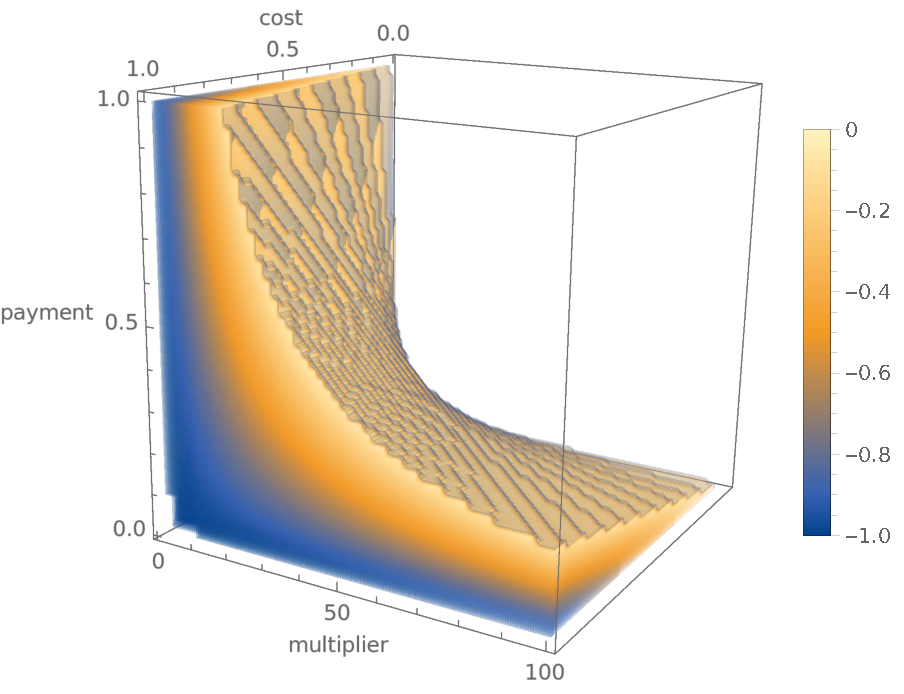
\includegraphics[width=\textwidth]{promise/figures/user-utility.pdf}
%     \caption{The utility for a user to pre-pay a certain number $m$ of payments $p$ depends on two factors: the cost for making the payment and requesting the service $c$ and the expected opportunity cost for locking a certain number of payments $\mathrm{E}[rmp]$. For this plot, we fix the expected return $r$ at $0.05$. The colored part of this plot represents the regions in which it is \emph{not} incentive compatible for a user to pre-pay depending on the cost, payment, and multiplier. The lower the cost for making a transaction, the smaller the multiplier should be. The higher the payment, the higher the payment, the smaller the multipler should be.}
%     \label{fig:user-decision}
% \end{figure}

\subsection{Incentive arguments}
\dom{Personal playground for now ;)}


Say preference for intermediary to cheat is $v$.
Provided deposit is $D_I < D_{min}$.
Without \sys, provided deposit is $D_{min}$.
Let's say $v = D_{min}$, i.e.\ 100\% collateralization ratio.

\subsubsection{Single-round game}
Assuming a protocol without \sys.
If Alice cheats, she gets $u = v - D_{min} = 0$.
If Alice is honest, she gets $u = p$.
Without \sys, Alice should not cheat in a single round game.

Assuming a protocol with \sys:
If Alice cheats, she gets $u = v - D_I > 0$
If Alice is honest, she gets $u = (\frac{\delta}{1+r})^{\tau} p$
For Alice not to cheat in a system with \sys in a single-round setting, we require:

\begin{equation}
    \big( \frac{\delta}{1+r} \big)^{\tau} p > v - D_I
\end{equation}

Consequences:
\begin{itemize}
    \item Safely reducing the initial collateral from $D_{min}$ to $D_I$ is bound to $D_I = D_{min} - (\frac{\delta}{1+r})^{\tau} p$.
    \item Assuming $\delta < 1$ and $r \geq 1$, the larger $\tau$, the less initial reduction is possible.
    \item The lower $\delta$ the less reduction.
    \item The higher $r$, the less reduction.
\end{itemize}

\subsubsection{Sequential game}
Assuming a protocol without \sys.
If Alice cheats, she gets $u = \sum_{t=0}^{\infty} \big( \frac{\delta}{1+r} \big)^{t} (v - D_{min}) = 0$.
If Alice is honest, she gets $u = \sum_{t=0}^{\infty} \big( \frac{\delta}{1+r} \big)^{t} p > 0$.
Without \sys, Alice should not cheat in a sequential game.

Assuming a protocol with \sys:
If Alice cheats, she gets $u = \sum_{t=0}^{\infty} \big( \frac{\delta}{1+r} \big)^{t} (v - D_{I}) > 0$
If Alice is honest, she gets $u = \sum_{t=0}^{\infty} \big( \frac{\delta}{1+r} \big)^{t} (\frac{\delta}{1+r})^{\tau} p$
For Alice not to cheat in a system with \sys in a single-round setting, we require:



% This modifies payoffs as follows. 

% \begin{equation}
% \label{eq:promise-quo_alice_honest}
% \Pi_A(A=H) = p - \mathrm{E}[r](D_{I}+p)
% \end{equation}

% where $\mathrm{E}[r](D_{I}-p)$ reflects the opportunity cost of locking the capital for one period.

% \begin{equation}
% \label{eq:promise-quo_alice_cheat}
% \Pi_A(A=C) = \Gamma_A - \mathrm{E}[r](D_{I}+p)-D_{base}
% \end{equation}

% Payoffs to Bob.

% \begin{equation}
% \label{eq:promise-quo_bob_alice_honest}
% \Pi_B(A=H) = \Gamma_B - p-c_L
% \end{equation}

% where $c_L<c$ denotes the effective per transaction cost for Bob, reflecting the average cost per transaction for n transactions, $\frac{c}{n}$.

% \begin{equation}
% \label{eq:promise-quo_bob_alice_cheat}
% \Pi_B(A=C) = -c_L
% \end{equation}

% \begin{figure}
%     \centering
%     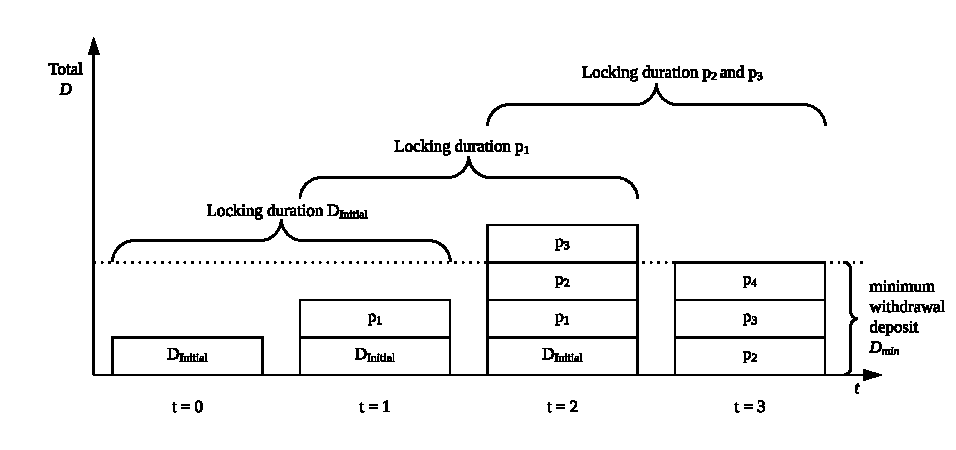
\includegraphics[width=\textwidth]{promise/figures/Promise.pdf}
%     \caption{\sys allows intermediaries to lock-up less initial deposit $D_I$ and use payments $p_i$ as additional deposit. The initial deposit and payments are locked for a period of time $\tau$. If the time period has passed and the agent has more collateral than the minimum requirement $D_{min}$, the agent can withdraw surplus collateral. In this example, at $t=0$ the intermediary Alice provided $D_I$ as the initial deposit, which is locked for two time steps (i.e.\ becomes free at $t=3$). At $t=1$, Bob pays Alice for executing a task with $p_1$ which is stored as additional collateral. At $t=2$, Alice receives two more payments from Bob, $p_2$ and $p_3$ which bring her total collateral above the minimum requirement $D_{min}$. At $t=4$ Alice is allowed to withdraw an amount equal to $D_I + p_1$ as both the locking period of these have passed and with $p_4$ Alice's overall collateral is at least equal to the minimum collateral requirement.}
%     \label{fig:promise}
% \end{figure}